\documentclass[11pt, oneside]{article}   	% use "amsart" instead of "article" for AMSLaTeX format

\usepackage{geometry}                		% See geometry.pdf to learn the layout options. There are lots.
\geometry{letterpaper}                   		% ... or a4paper or a5paper or ... 

\usepackage[parfill]{parskip}    		% Activate to begin paragraphs with an empty line rather than an indent
\usepackage{graphicx}				% Use pdf, png, jpg, or eps§ with pdflatex; use eps in DVI mode
\graphicspath{{images/}}
								% TeX will automatically convert eps --> pdf in pdflatex
\usepackage{amsmath}


\title{The Cable Project}
\author{Elise Niedringhaus, Sarah Liddle and Darice Guittet}
%\date{}							% Activate to display a given date or no date

\begin{document}
\maketitle
\section{Traveling Wave Solutions to the Cable Equation}
The local voltage of the neural membrane and the behavior of the ion currents depend on one another. One way to explore the effects of this dependency is to choose an ionic current $f(v(x,t))$ that results in a bistable system.In this context, bistable means the membrane has two stable equilibria described by an active and an inactive state. This bistable system yields traveling wave solutions to the cable equation. These two states can be implemented in the equation using the Heaviside step nonlinearity, which is defined to be $f(v)=-v+H(v-\theta)$.\\

\begin{equation}
  H(v-\theta)=\begin{cases}
    0, & \text{when $v<\theta$}.\\
    1, & \text{when $v>\theta$}.
  \end{cases}
\end{equation}


\subsection{Homogeneous Solutions}
First, look for homogeneous solutions that are constant in both space and time, denoted $v(x,t)=\overline{v}$. The two possible homogeneous solutions of $\frac{\partial v(x,t)}{\partial t}=\frac{\partial ^2 v(x,t)}{\partial x^2}-v(x,t)+H(v-\theta)+J_{ext}(x,t)$ are found by taking the appropriate derivatives of $v(x,t)=\overline{v}$ and substituting them into the partial differential equation. 
$$\frac{\partial \overline{v}(x,t)}{\partial t}=0$$
$$\frac{\partial ^2 \overline{v}(x,t)}{\partial x^2}=0$$
$$0=0-\overline{v}+H(\overline{v}-\theta)$$
When $\overline{v}>\theta$, $0=-\overline{v}+1$. When $\overline{v}<\theta$, $0=-\overline{v}+0$

Thus, the two homogeneous solutions are 
$$\overline{v}^+=1\text{, when $\overline{v}>\theta$}$$
$$\overline{v}^-=0\text{, when $\overline{v}<\theta$}$$
In order for both of these solutions to exist, it must be true that ????

\subsection{Change of Variables and Boundary Conditions}
Since the ratio of the diameter to the length of a neuronal axon is very small, we will impose the assumption that they are infinitely long cables with $x\in (-\infty,\infty)$. Furthermore, we will impose the following boundary conditions
$$\lim_{x\to\infty} \frac{\partial v(x,t)}{\partial x}=0 \text{ and } \lim_{x\to-\infty} \frac{\partial v(x,t)}{\partial x}=0.$$
Physically, these boundary conditions are significant because as x approaches the outer ends of the neurons, the voltage should not be changing. ???? \\
In order to find traveling wave solutions, we can apply the change of variables $v(x,t)=V(\xi),$ where $\xi=x-ct$, to the partial differential equation. Furthermore, assume that the external current $J_{ext}(x,t)$ is $0$. The new second order ordinary differential equation is 
\begin{equation}
\label{second order ODE}
-cV'(\xi)=V''(\xi)-V(\xi)+H(V(\xi)-\theta)
\end{equation}

In order to solve for traveling wave solutions, we assume that the solution is a traveling front solution that decreases as $\xi$ increases. So, define $V(\xi)>\theta$ when $\xi<0$ and that $V(\xi)<\theta$ when $\xi>0$. ??? re explain this??? The Heaviside step nonlinearity is now defined as 

\begin{equation}
  H(V(\xi)-\theta)=\begin{cases}
    0, & \text{when $V(\xi)<\theta$}.\\
    1, & \text{when $V(\xi)>\theta$}.
  \end{cases}
\end{equation}

Equation \ref{second order ODE} can now be decomposed into the following two second order ordinary differential equations for $V_1(\xi)$ and $V_2(\xi)$.
\begin{equation}
\label{ODE1}
-cV_1'(\xi)=V_1''(\xi)-V_1(\xi) \text{ when  $\xi \in (0,\infty)$}
\end{equation}

\begin{equation}
\label{ODE2} 
-cV_2'(\xi)=V_2''(\xi)-V_2(\xi)+1 \text{ when $\xi \in (-\infty,0)$.}
\end{equation}

In order to ensure the solutions to equations \ref{ODE1} and \ref{ODE2} are physically realistic, we must impose boundary conditions. $V(\xi)$ must approach the homogeneous solution as $\xi$ approaches $\pm \infty$. Also, the two solutions and their first derivatives must match at $\xi=0$. Physically, this is because we want to model the voltage, which should be continuously differentiable. Mathematically, the boundary conditions are described by\\
$$\lim_{\xi\to-\infty} \frac{d V_1(\xi)}{d \xi}=0$$
$$\lim_{\xi\to\infty} \frac{d V_2(\xi)}{d \xi}=0$$
$$\lim_{\xi\to-\infty} V_1(\xi)=1$$
$$\lim_{\xi\to\infty} V_2(\xi)=0$$
$$V_1(0)=V_2(0)$$
$$\frac{d V_1}{d \xi}(0)=\frac{d V_2}{d \xi}(0)$$


\subsection{Solving for Traveling Wave Solutions}

Equation \ref{ODE1} is a homogeneous ordinary differential equation. The corresponding characteristic equation, $r^2+cr-1=0$, has roots of  $r=\frac{-c \pm \sqrt{c^2+4}}{2}$. The general solution to equation \ref{ODE1} is 
\begin{equation}
\label{ODE1 general solution}
V_{1}=c_1 e^{\frac{1}{2}(-c+\sqrt{c^2+4})\xi}+c_2e^{-\frac{1}{2}(c+\sqrt{c^2+4})\xi}, \xi \in (0,\infty)
\end{equation}

Equation \ref{ODE2} is not homogeneous, but can be solved using the method of undetermined coefficients. First, the homogeneous solution is obtained by solving $cV_2'(\xi)=V_2''(\xi)-V_2(\xi)$ for $V_2$. The homogeneous solution is
$$V_{2,h}=c_3 e^{\frac{1}{2}(-c+\sqrt{c^2+4})\xi}+c_4 e^{-\frac{1}{2}(c+\sqrt{c^2+4})\xi}$$
Now, we guess a particular solution of the form $V_{2,p}=A$. Plugging $V_{2,p}$ into equation \ref{ODE2} yields 
$$-c(0)=0-A+1$$
$$A=1$$ 
$$V_{2,p}=1$$
Thus, the solution to equation \ref{ODE2} is 
\begin{equation}
\label{ODE2 general solution}
V_{2}=c_3 e^{\frac{1}{2}(-c+\sqrt{c^2+4})\xi}+c_4 e^{-\frac{1}{2}(c+\sqrt{c^2+4})\xi}+1, \xi \in (-\infty,0)
\end{equation}
Next, use the boundary conditions to eliminate the unknown coefficients from equations \ref{ODE1 general solution} and \ref{ODE2 general solution}. 
$$\lim_{\xi\to\infty} \frac{d V_1(\xi)}{d \xi}=0\Rightarrow c_1=0$$
$$\lim_{\xi\to-\infty} \frac{d V_2(\xi)}{d \xi}=0\Rightarrow c_4=0$$
$$V_1(0)=V_2(0)\Rightarrow c_2=c_3+1$$
$$\frac{d V_1}{d \xi}(0)=\frac{d V_2}{d \xi}(0)\Rightarrow -\frac{1}{2}(c+\sqrt{c^2+4}) c_2= \frac{1}{2}(-c+\sqrt{c^2+4})c_3$$ 
The solution to this linear system of equations is $c_1=0, c_2=\frac{-c+\sqrt{c^2+4}}{2\sqrt{c^2+4}}, c_3=\frac{-c-\sqrt{c^2+4}}{2\sqrt{c^2+4}}$, and $c_4=0$.\\
The solution to equation \ref{ODE1} is 
\begin{equation}
\label{ODE1 solution}
V_1(\xi)=\frac{-c+\sqrt{c^2+4}}{2\sqrt{c^2+4}}e^{-\frac{1}{2}(c+\sqrt{c^2+4})\xi},\xi \in (0,\infty).
\end{equation}
The solution to equation \ref{ODE2} is
\begin{equation}
\label{ODE2 solution}
V_2(\xi)=\frac{-c-\sqrt{c^2+4}}{2\sqrt{c^2+4}}e^{\frac{1}{2}(-c+\sqrt{c^2+4})\xi}+1,\xi \in (-\infty,0).
\end{equation}


\subsection{Analysis of the Traveling Wave Solution}
In order to understand the relationship between the speed of the traveling front, c, and the threshold value $\theta$, apply the threshold condition that $V(0)=\theta$. Application of this threshold condition to the traveling wave solutions gives $\frac{-c}{2\sqrt{c^2+4}}+\frac{1}{2}=\theta$.
$$\frac{-c}{\sqrt{c^2+4}}+1=2\theta$$
$$\frac{-c}{\sqrt{c^2+4}}=2\theta-1$$
$$\frac{c^2}{c^2+4}=(2\theta-1)^2$$
$$c^2(1-(2\theta-1)^2)=4(2\theta-1)^2$$
$$c=\sqrt{\frac{4(2\theta-1)^2}{1-(2\theta-1)^2}}$$
$$c=\sqrt{\frac{-(2\theta-1)^2}{\theta^2-\theta}}$$

\begin{figure}[H]
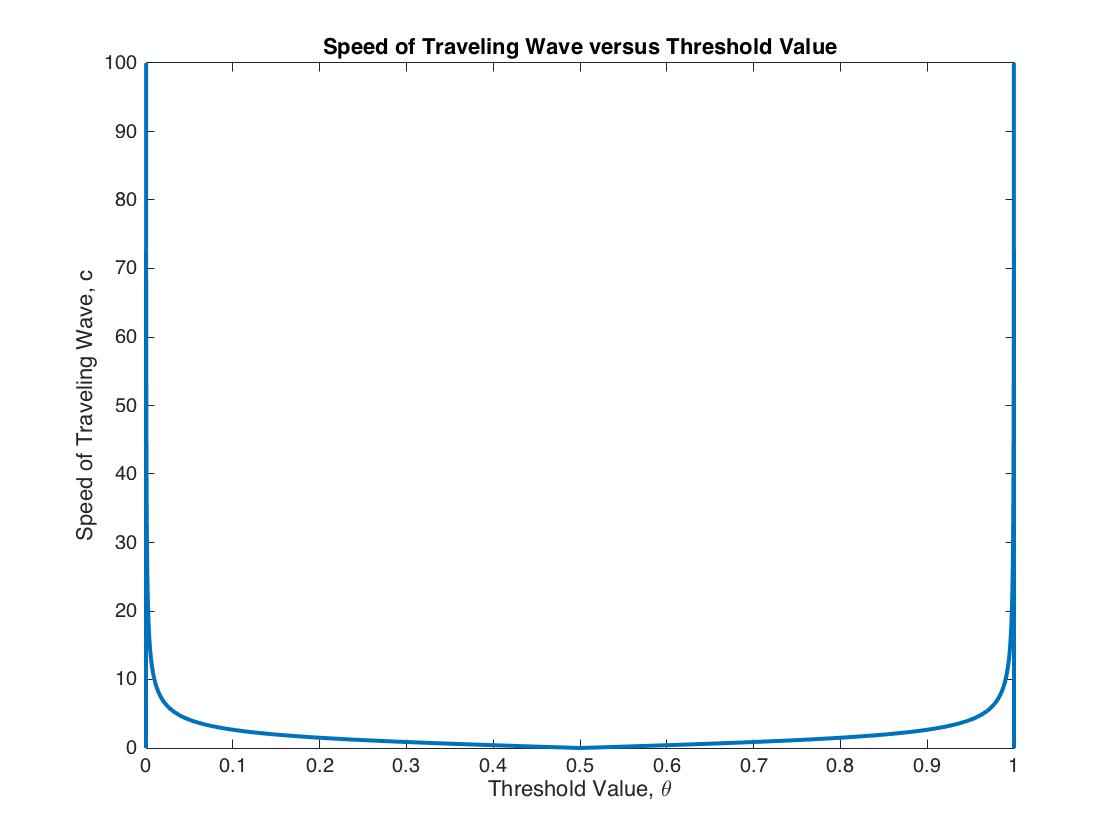
\includegraphics[width=0.7\textwidth]{cVStheta.jpg}
\caption{test test}
\label{test}
\end{figure}

\subsection{2f}
Partial differential equation: 
\begin{equation}
\label{uh}
\frac{\partial v}{\partial t}=\frac{\partial ^2 v}{\partial x^2}+f(v(x,t))
\end{equation}
where $f(v)=-v+H(v-\theta)$.\\
In order to analyze the stability of the traveling wave solution found, consider the solution $v(x,t)=V(\xi)+\epsilon\psi(\xi,t)$, where $0 < \epsilon <<1$ and $\psi(\xi,t)$ represents a small perturbation to the traveling wave solution. 
$$\frac{\partial v}{\partial t}=\frac{\partial\xi}{\partial t}\frac{dV}{d\xi}+\epsilon(\frac{\partial \psi}{\partial \xi}\frac{\partial \xi}{\partial t}+\frac{\partial \psi}{\partial t})$$
$$\Rightarrow \frac{\partial v}{\partial t}=-c\frac{dV}{d\xi}+\epsilon(-c\frac{\partial \psi}{\partial \xi}+\frac{\partial \psi}{\partial t})$$
$$\frac{\partial v}{\partial x}=\frac{\partial \xi}{\partial x}\frac{dV}{d\xi}+\epsilon\frac{\partial\xi}{\partial x}\frac{\partial\psi}{\partial\xi}$$
$$\Rightarrow \frac{\partial v}{\partial x}=\frac{dV}{d\xi}+\epsilon\frac{\partial\psi}{\partial\xi}$$
$$\frac{\partial^2 v}{\partial x^2}=\frac{\partial \xi}{\partial x}\frac{d^2V}{d\xi^2}+\epsilon\frac{\partial^2\psi}{\partial\xi^2}\frac{\partial \xi}{\partial x}$$
$$\Rightarrow \frac{\partial^2 v}{\partial x^2}=\frac{d^2V}{d\xi^2}+\epsilon\frac{\partial^2\psi}{\partial\xi^2}$$
Equation \ref{uh} can be rewritten as 
\begin{equation}
\label{frewritten}
-c\frac{dV(\xi)}{d\xi}+\epsilon(-c\frac{\partial \psi(\xi,t)}{\partial \xi}+\frac{\partial \psi(\xi,t)}{\partial t})=\frac{d^2V(\xi)}{d\xi^2}+\epsilon\frac{\partial^2\psi(\xi,t)}{\partial\xi^2}+f(V(\xi)+\epsilon\psi(\xi,t))
\end{equation}
where $f(V(\xi)+\epsilon\psi)=-(V(\xi)+\epsilon\psi(\xi,t))+H(V(\xi)+\epsilon\psi(\xi,t)-\theta)$.\\

Analysis of equation \ref{frewritten} can be simplified by using the Taylor expansion of $f(V(\xi)+\epsilon\psi)$ with respect to $\epsilon$, about $\epsilon=0$.
$$f(V(\xi)+\epsilon\psi)\approx f(V(\xi)+\epsilon\psi)\Big|_{\epsilon=0}+\Bigg(\frac{\partial f(V(\xi)+\epsilon\psi)}{\partial \epsilon}\Big|_{\epsilon=0}\Bigg)\epsilon+O(\epsilon ^2)$$
$$f(V(\xi)+\epsilon\psi)\approx f\big(V(\xi)\big)+\big(-\psi(\xi,t)+\psi(\xi,t) \delta(V(\xi)-\theta)\big)\epsilon$$
$$f(V(\xi)+\epsilon\psi)\approx -V(\xi)+H(V(\xi)-\theta)+\psi(\xi,t)\epsilon\big(-1+\delta(V(\xi)-\theta)\big)$$
Equation \ref{frewritten} becomes
$$-c\frac{dV(\xi)}{d\xi}+\epsilon(-c\frac{\partial \psi(\xi,t)}{\partial \xi}+\frac{\partial \psi(\xi,t)}{\partial t})=\frac{d^2V(\xi)}{d\xi^2}+\epsilon\frac{\partial^2\psi(\xi,t)}{\partial\xi^2}-V(\xi)+H(V(\xi)-\theta)+\psi(\xi,t)\epsilon\big(-1+\delta(V(\xi)-\theta)\big)$$
In order to analyze the long term behavior of the disturbance, look only at the terms involving $\psi$ and $\epsilon$. The partial differential equation that models the behavior of the perturbation is:
$$\epsilon(-c\frac{\partial \psi(\xi,t)}{\partial \xi}+\frac{\partial \psi(\xi,t)}{\partial t})=\epsilon\frac{\partial^2\psi(\xi,t)}{\partial\xi^2}+\psi(\xi,t)\epsilon\big(-1+\delta(V(\xi)-\theta)\big)$$
$$-c\frac{\partial \psi(\xi,t)}{\partial \xi}+\frac{\partial \psi(\xi,t)}{\partial t}=\frac{\partial^2\psi(\xi,t)}{\partial\xi^2}+\psi(\xi,t)\big(-1+\delta(V(\xi)-\theta)\big)$$
In order to further understand the behavior of the perturbation, solve the partial differential equation to the left and the right of $V(\epsilon)=\theta$. The governing equation for $V(\xi)\neq\theta$ is 
\begin{equation}
\label{psiPDE}
-c\frac{\partial \psi(\xi,t)}{\partial \xi}+\frac{\partial \psi(\xi,t)}{\partial t}=\frac{\partial^2\psi(\xi,t)}{\partial\xi^2}-\psi(\xi,t)
\end{equation}
since $\delta(V(\xi)-\theta)=0$ whenever $V(\xi)\neq\theta$. This equation can be solved using separation of variables, which means solutions should have the form of $\psi(\xi,t)=F(\xi)G(t)\neq0$.
This proposed solution must satisfy the partial differential equation in equation \ref{psiPDE}.
$$-cG(t)\frac{dF(\xi)}{d\xi}+F(\xi)\frac{dG(t)}{dt}=G(t)\frac{d^2F(\xi)}{d\xi^2}-F(\xi)G(t)$$
$$-c\frac{1}{F(\xi)}\frac{dF}{d\xi}+\frac{1}{G(t)}\frac{dG}{dt}=\frac{1}{F(\xi)}\frac{d^2F(\xi)}{d\xi^2}-1$$
$$\frac{1}{F(\xi)}\frac{d^2F(\xi)}{d\xi^2}+c\frac{1}{F(\xi)}\frac{dF}{d\xi}-1=\frac{1}{G(t)}\frac{dG}{dt}=\lambda$$
$$\frac{1}{G(t)}\frac{dG}{dt}=\lambda$$
Thus, the time dependence of $\psi(\xi,t)$ is described by $G(t)=C_1e^{\lambda t}$. Now, consider $\frac{1}{F(\xi)}\frac{d^2F(\xi)}{d\xi^2}+c\frac{1}{F(\xi)}\frac{dF}{d\xi}-1=\lambda$
$$\frac{d^2F(\xi)}{d\xi^2}+c\frac{dF(\xi)}{d\xi}-F(\xi)(1+\lambda)=0$$
The three cases to consider are $\lambda=0$, $\lambda<0$ and $\lambda>0$. When $\lambda=0$, $\frac{d^2F(\xi)}{d\xi^2}+c\frac{dF(\xi)}{d\xi}-F(\xi)=0$ gives $F(\xi)=Ae^{\frac{1}{2}(-c+\sqrt{c^2+4})\xi}+Be^{-\frac{1}{2}(c+\sqrt{c^2+4})\xi}$.
$v(x,t)=V(\xi)+\epsilon\psi(\xi,t)$







\end{document}  